\chapter{System Design and Methodology}

\section{Arena Setup and Coordinate System}

The experimental arena is a domestic garage measuring 6230 mm in the X direction, 3050 mm in the Y direction, and 2950 mm in the Z direction. The world-frame origin is defined at the North-East floor corner. The \textbf{X-axis} points from the North wall toward the South wall, the \textbf{Y-axis} points from the East wall toward the West wall, and the \textbf{Z-axis} points vertically upward.

All coordinates in this thesis are reported in millimetres. The main operating volume for the athlete lies approximately between X = 2500 mm and X = 5000 mm, where the four camera frusta overlap most reliably.

\begin{table}[htbp]
\centering
\caption{Camera positions in world-frame coordinates (mm)}
\label{tab:3_1}
\begin{tabular}{|c|c|c|c|p{3.5cm}|}
\hline
\textbf{Camera} & \textbf{X (mm)} & \textbf{Y (mm)} & \textbf{Z (mm)} & \textbf{Description} \\
\hline
CamNorth & 50 & 1100 & 2260 & North wall, central height \\
\hline
CamEast & 1620 & 50 & 2120 & East wall, near North end \\
\hline
CamWest & 1600 & 2970 & 2170 & West wall, near North end \\
\hline
CamSouth & 6180 & 1530 & 2270 & South wall, central \\
\hline
\end{tabular}
\end{table}

The cameras are mounted near the ceiling and perimeter walls to maximise overlapping views of the central volume. The intended operating condition is that at least three cameras observe the athlete's target joint. The repository's current geometry is represented by the \texttt{arena\_fixed} calibration bundle, which fixes the world-frame convention and binds the active intrinsics, extrinsics, arena dimensions, correction models, and evaluation reports.

Twenty-four AprilTag markers (IDs 0--23; 21.5 cm $\times$ 21.5 cm) are attached to the arena walls at measured world-frame positions. These markers support extrinsic calibration as described in Section 3.5.

\section{Hardware Architecture}

\subsection{Cameras}

The vision system uses four Hikvision DS-E12 USB webcams at 1280 $\times$ 720 px and a target capture rate of 15 FPS. These are fixed-focus commodity cameras without hardware synchronisation. Their low cost is central to the thesis objective, but it also imposes constraints: rolling capture timing, lens distortion, and limited optics increase the importance of calibration and robust filtering.

\subsection{Ball Launching Machine}

The BLM consists of two counter-rotating wheel motors for ball projection, two stepper-driven axes for pitch and yaw, and a ball feed mechanism controlled by \texttt{shoot} and \texttt{reload} commands. Wheel speed determines the approximate launch speed; differential wheel speed can introduce spin. The pitch and yaw steppers orient the launcher toward the selected target.

The launch origin is modelled as a fixed world-frame point,
$B = (600, 1560, 500)$ mm, near the North side of the arena and centred in Y. The launcher reference direction points along the positive X-axis toward the athlete region.

\begin{figure}[htbp]
\centering
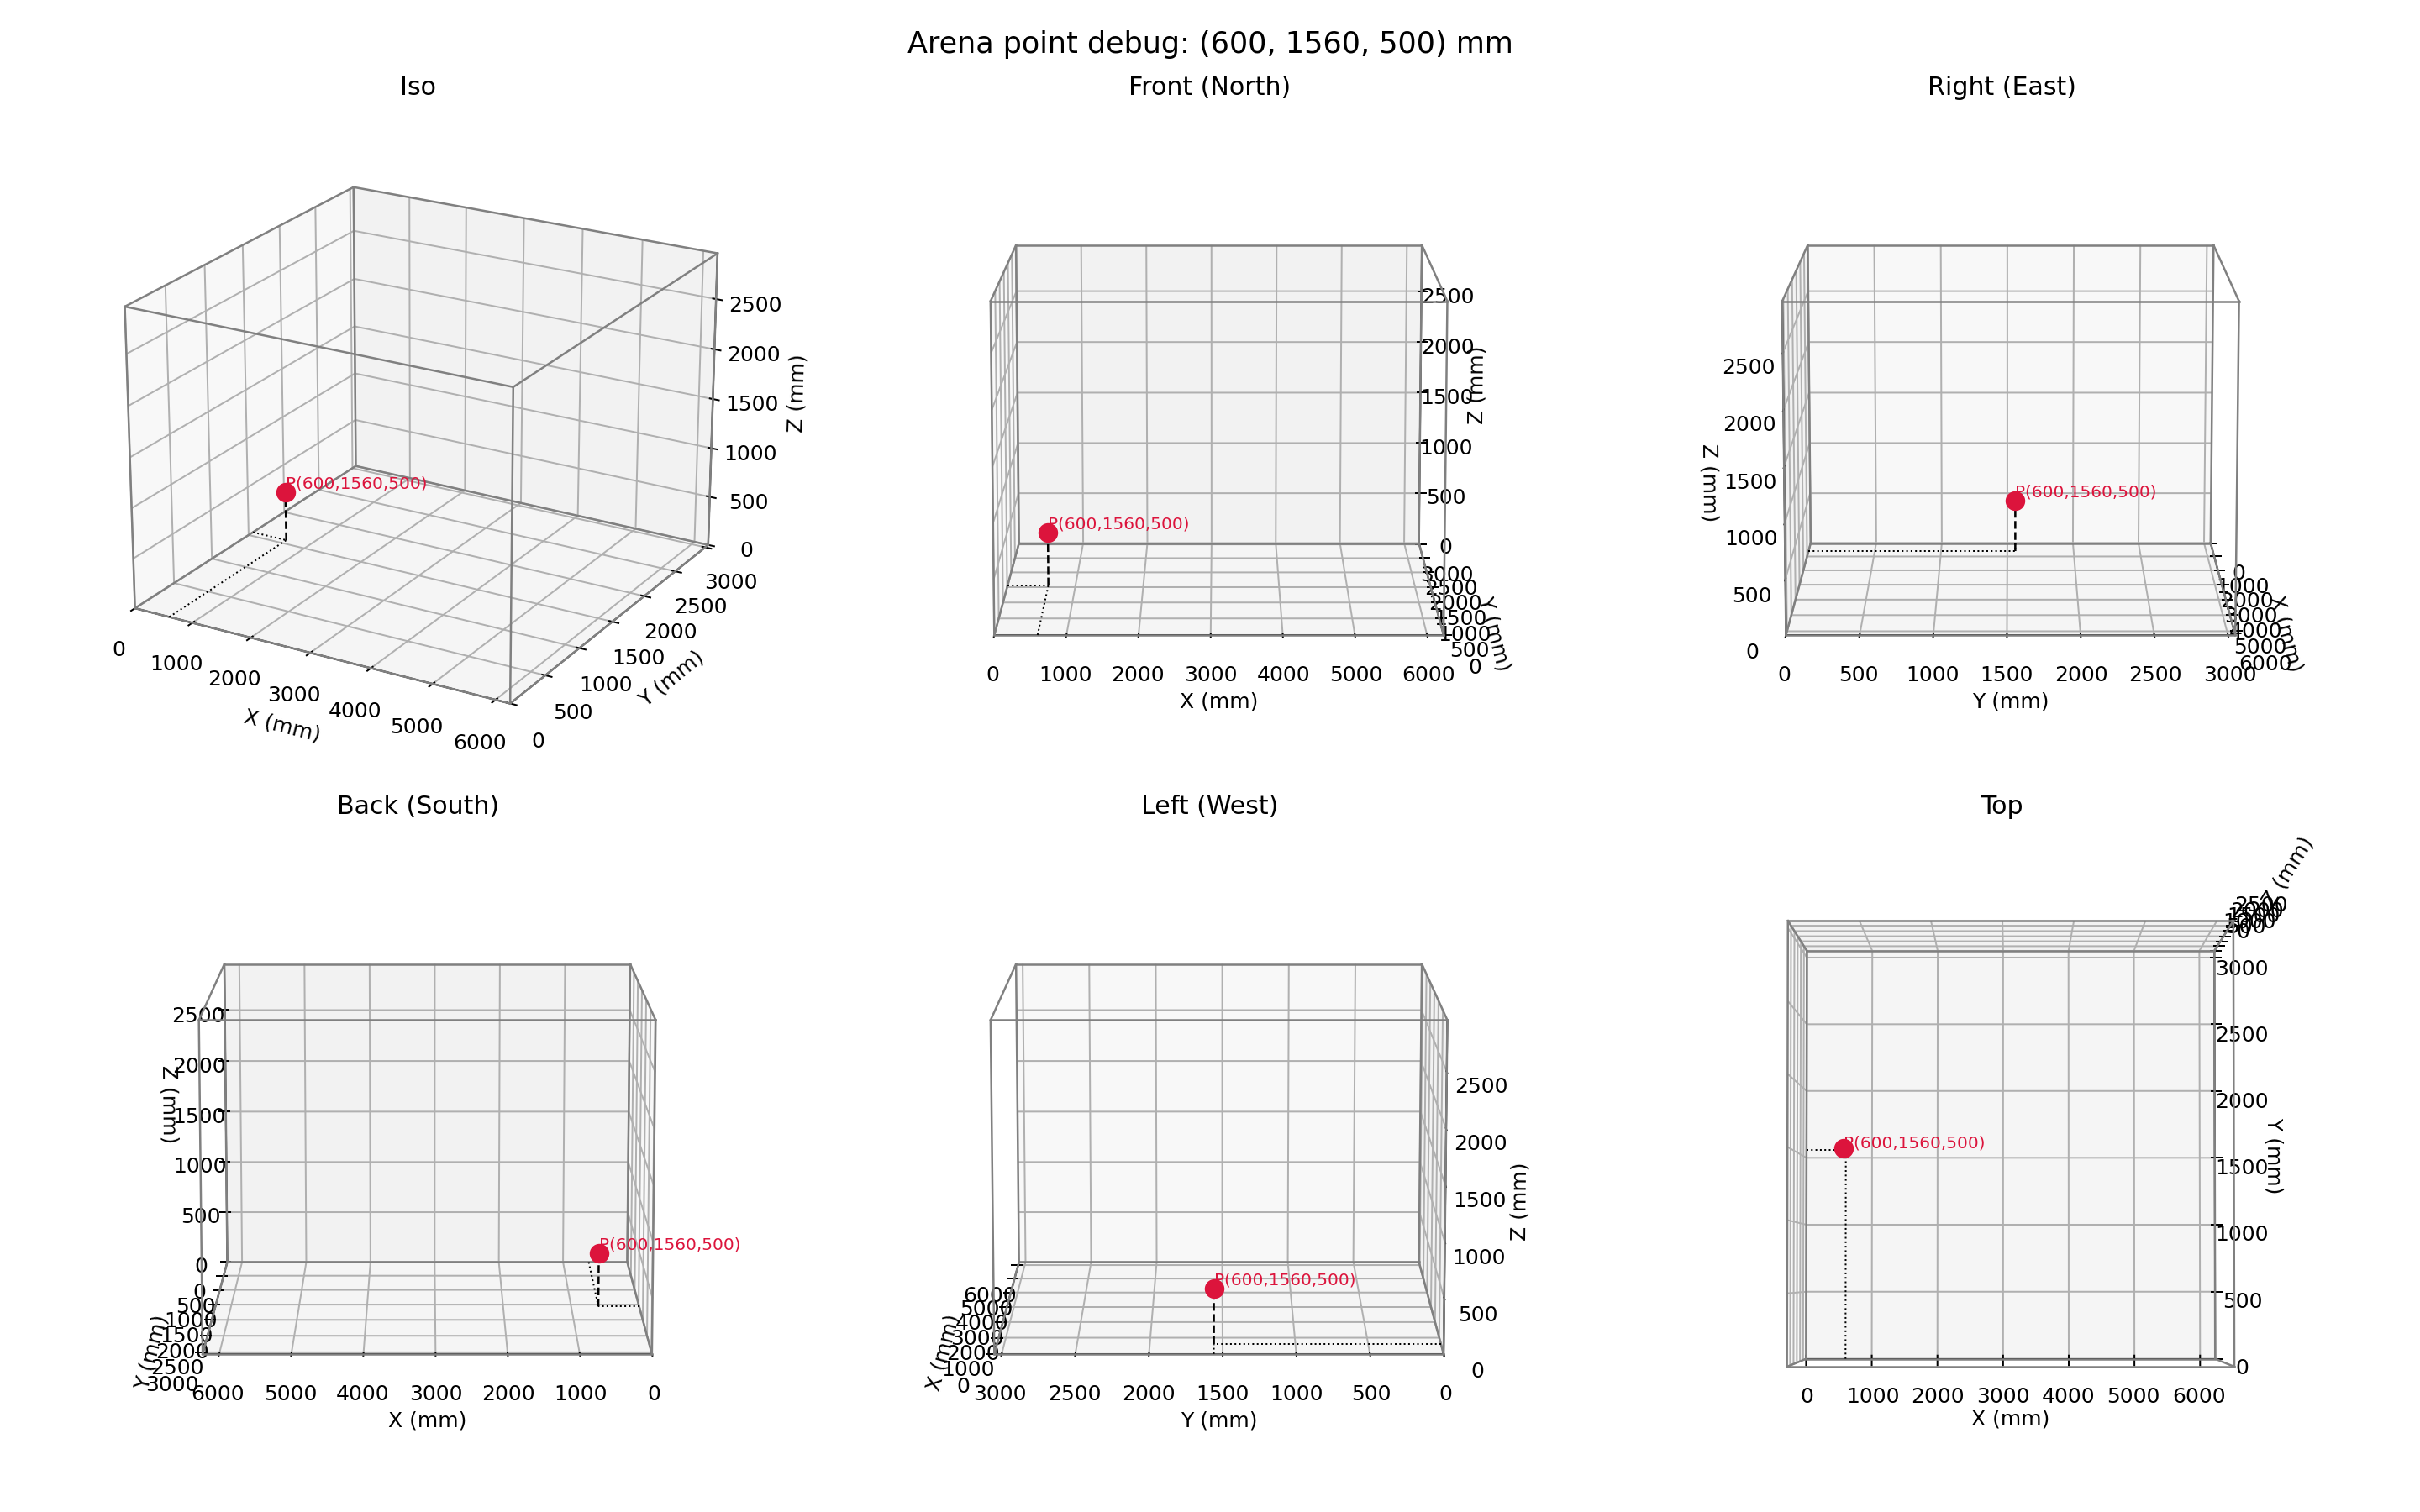
\includegraphics[width=0.9\textwidth]{figures/blm_anchor_600_1560_500_multiview}
\caption{World-frame visualisation of the BLM anchor point at $(600, 1560, 500)$ mm projected into the calibrated multi-camera arena. The figure is used to clarify coordinate alignment and launcher placement; it is not a closed-loop firing result.}
\label{fig:3_blm_anchor}
\end{figure}

\subsection{ESP32 Microcontroller}

An ESP32 microcontroller receives serial commands from the host PC and translates them into motor-control actions. The low-level command set is shown in Table~\ref{tab:3_2}.

\begin{table}[htbp]
\centering
\caption{BLM low-level serial command set}
\label{tab:3_2}
\begin{tabularx}{\textwidth}{|l|l|X|}
\hline
\textbf{Command} & \textbf{Syntax} & \textbf{Effect} \\
\hline
set & \texttt{set V H WL WR} & Set vertical angle V, horizontal angle H, left wheel speed WL, and right wheel speed WR \\
\hline
shoot & \texttt{shoot} & Trigger one ball ejection cycle \\
\hline
reload & \texttt{reload} & Retract the ball feed mechanism for the next cycle \\
\hline
center & \texttt{center} & Return the pitch and yaw axes to logical zero \\
\hline
stop & \texttt{stop} & Stop motor activity immediately \\
\hline
setzero & \texttt{setzero} & Register the current mechanical pose as logical zero \\
\hline
\end{tabularx}
\end{table}

The current firmware implementation, \path{control_12_full.ino}, uses a 921600-baud serial command path and also exposes a BLE interface for manual interaction. The feeder is implemented as a finite-state machine with \texttt{IDLE}, \texttt{SHOOTING}, \texttt{RETRACTING}, and \texttt{DISPENSING} states. The \texttt{shoot} command waits until both measured wheel speeds exceed the configured feed threshold before advancing the pusher, while \texttt{reload} retracts the pusher and dispenses a ball until a limit switch or timeout condition is reached. These firmware details support the staged integration protocol, but they do not by themselves establish projectile accuracy.

\subsection{PC--ESP32 Architecture Split}

High-level computation runs on the host PC: camera capture, detection, pose estimation, triangulation, filtering, ballistic solving, safety gating, and decision logging. The ESP32 executes only low-level motor commands. This split keeps GPU-heavy perception on the PC, simplifies firmware, and allows targeting logic to be modified without reflashing the controller.

\section{Software Architecture and Pipeline Overview}

The pipeline proceeds through seven stages. Stage 1 is \textbf{multi-camera capture}, where the four camera frames are acquired at the configured resolution. Stage 2 is \textbf{ball detection}, where a YOLO-based detector returns ball bounding boxes and confidence scores. Stage 3 is \textbf{human pose estimation}, where a COCO-format pose backend returns 17 keypoints and per-keypoint confidences. Stage 4 is \textbf{3D triangulation}, where valid 2D observations are combined through the DLT/SVD solver to estimate ball and joint coordinates in the world frame. Stage 5 is \textbf{filtering}, where outlier rejection and smoothing are applied. Stage 6 is \textbf{ballistic solving}, where the selected target joint is converted into pitch, yaw, and wheel-speed commands. Stage 7 is \textbf{actuation or logging}, where commands are either sent to the ESP32 under enabled safety conditions or written to a JSONL log during dry-run tests.

The implementation uses Python 3.10. Key libraries include OpenCV \cite{ref27} for camera I/O and calibration, Ultralytics YOLO \cite{ref14} for ball detection, an open-source pose-estimation backend \cite{ref17} for COCO-format keypoints, NumPy \cite{ref28} and SciPy \cite{ref29} for numerical computation, and Matplotlib/OpenCV-based utilities for visualisation. The local repository contains both evaluation scripts and performance-oriented runtime scripts; this thesis reports only the evaluation results documented in the ground-truth folders.

\begin{figure}[htbp]
\centering
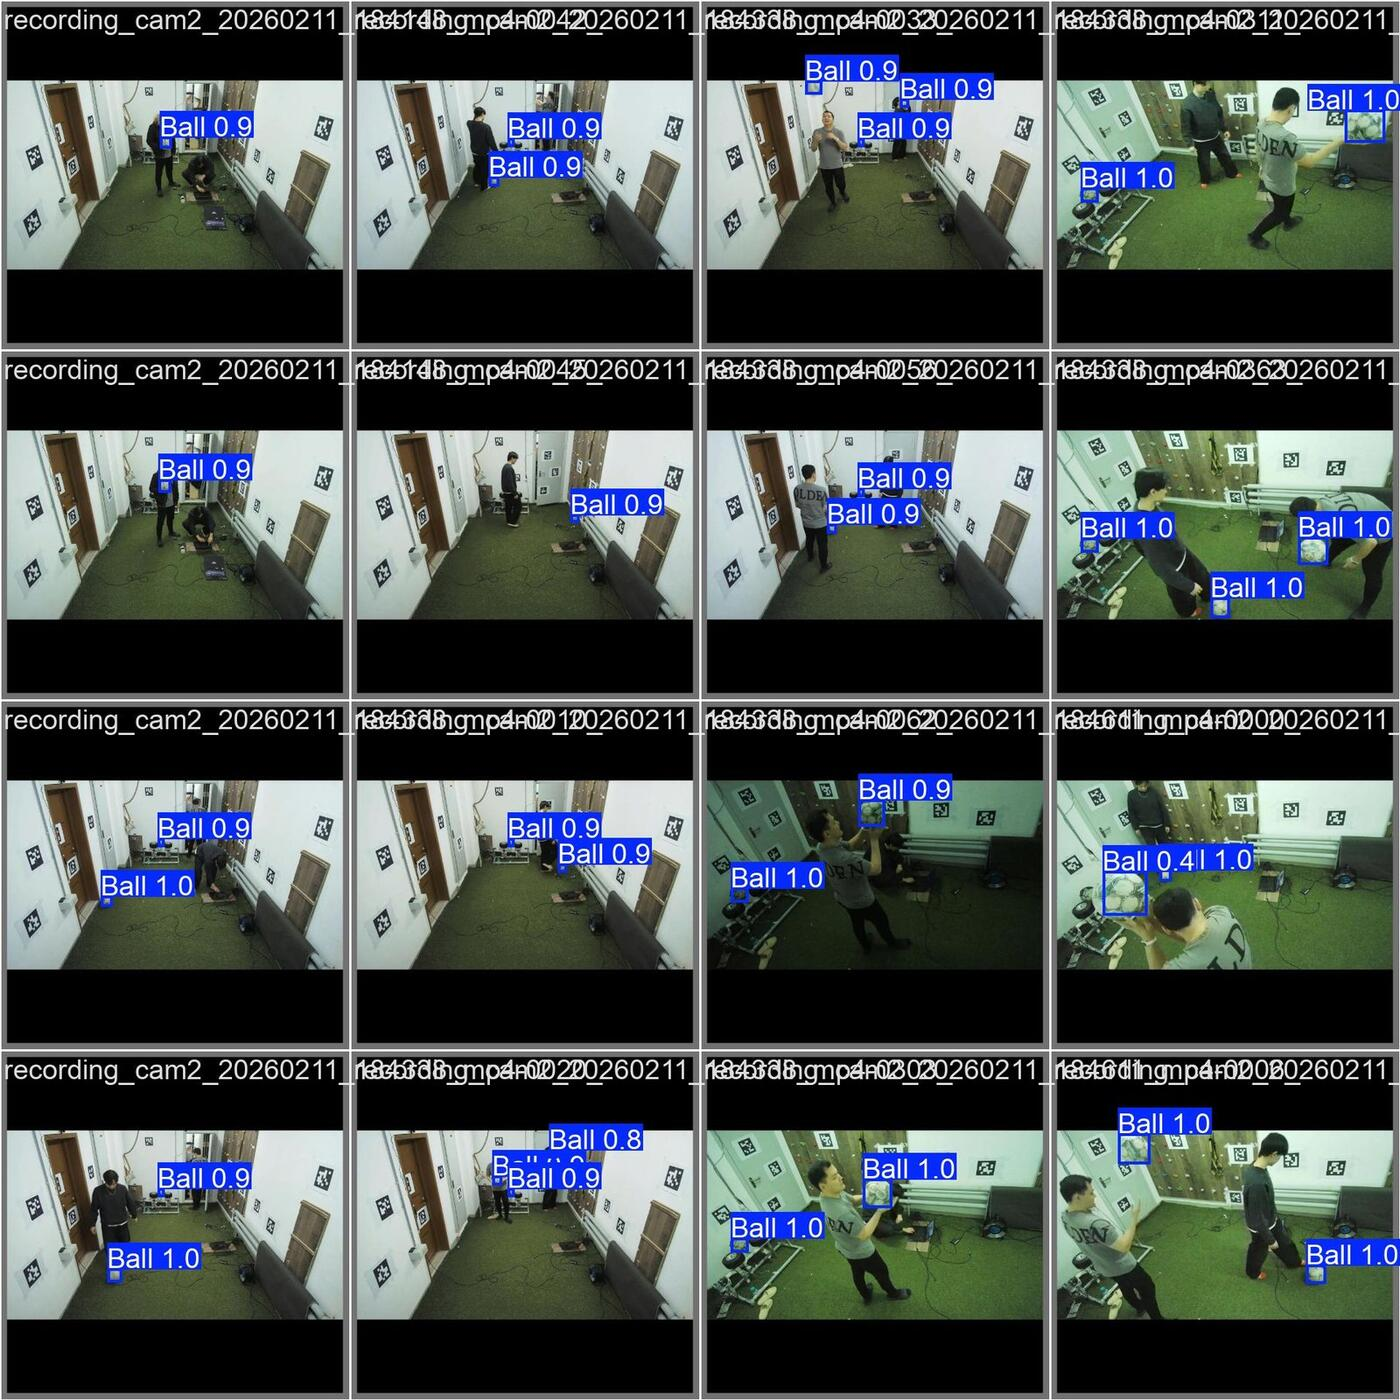
\includegraphics[width=0.9\textwidth]{figures/smoke_test_frame_1}
\caption{Live 4-camera arena view showing ball detection, human pose overlay, and 3D triangulated outputs during system operation.}
\label{fig:3_3}
\end{figure}

\section{Intrinsic Calibration Pipeline}

\subsection{Board Specification and Detection}

A ChArUco board with 5 columns and 7 rows is used for intrinsic calibration. The embedded ArUco markers provide identifiable corners even when the board is only partly visible. The auto-capture script monitors all four camera streams and saves calibration frames when enough ChArUco corners are detected stably. This reduces operator timing error and helps collect a more consistent calibration set.

\subsection{Calibration Procedure}

Each camera is calibrated independently at the same 1280 $\times$ 720 resolution used during operation. OpenCV \cite{ref27} estimates the intrinsic matrix $K$ and distortion coefficients ($k_1$, $k_2$, $p_1$, $p_2$, $k_3$) by minimising reprojection error over the collected calibration frames. Approximately 30 valid frames per camera are targeted, and frames with insufficient corner detections are discarded.

Calibrating at the operating resolution is important because resizing images after calibration requires corresponding rescaling of focal lengths and principal point. Avoiding this extra transformation reduces one source of systematic triangulation error.

\subsection{Output and Validation}

The calibration outputs are stored as JSON files in \path{garage_lab_combined/cal/intrinsics/}. Per-camera reprojection error is used as a quality indicator. The values are sufficient for prototype-level triangulation, but they are not the only determinant of 3D accuracy; extrinsic calibration, camera geometry, and keypoint quality remain dominant error sources.

\section{Extrinsic Calibration Pipeline}

\subsection{AprilTag Detection}

The AprilTag wall grid provides known 3D corner points. The robust extrinsic calibration script detects visible tags in captured frames and constructs 2D--3D correspondences between image tag corners and measured world-frame tag positions.

\subsection{Robust PnP Optimisation}

For each camera, the pose $(R, T)$ is estimated using PnP with iterative refinement. A sigma-clipping stage removes tag-corner observations whose reprojection residuals are inconsistent with the rest of the detected set. The resulting rotation and translation define the camera pose in the shared world frame.

\subsection{Overlay Validation}

Extrinsic quality is checked visually by reprojecting known AprilTag corners into each camera image using the estimated $(K, R, T)$ parameters. When reprojected corners align with detected corners across the camera views, the calibration is accepted for the session. This visual check is necessary because a low average reprojection error can still hide a wrong world-frame convention or a physically inconsistent tag measurement.

\section{Multi-Camera Synchronisation}

The Hikvision cameras do not provide hardware synchronisation. For recorded sessions, software synchronisation is performed using a flashlight marker: a brief brightness spike is created at the beginning of the recording and detected in all camera streams. Frames are then aligned by the spike index.

For static ground-truth holds of 3--4 seconds, synchronisation error of a few frames is acceptable because the target is stationary during the measurement window. For dynamic motion, temporal offset directly affects triangulation: if camera frames correspond to different physical instants, the reconstructed point can be displaced along the direction of motion. This limitation is one reason why the dynamic clips in Chapter 5 are interpreted as qualitative tracking checks rather than complete closed-loop moving-target validation.

\section{3D Triangulation}

\subsection{Ball Triangulation}

For each frame in which the ball is detected in at least two cameras with confidence above the configured threshold, the centre of each 2D bounding box is combined with the corresponding camera projection matrix. The DLT method constructs a matrix $A$ such that the homogeneous 3D point $P$ satisfies $A \cdot P = 0$ in the least-squares sense. SVD returns the estimated $P$ as the right singular vector corresponding to the smallest singular value \cite{ref1}.

\subsection{Pose Joint Triangulation}

For each COCO keypoint, the same triangulation method is applied to 2D joint detections whose confidence exceeds the threshold. A higher camera-count requirement is used for joints than for the ball because human keypoints are more sensitive to appearance ambiguity and self-occlusion. The right knee, right hip, and left shoulder are then extracted as target candidates for the BLM.

\subsection{Quality Filtering}

Two quality filters are applied after triangulation.

\textbf{Reprojection error check:} The estimated 3D point is projected back into each contributing camera. If the pixel error between the projected point and the original 2D observation exceeds the configured threshold, that estimate is rejected as an outlier.

\textbf{EMA smoothing:} Accepted 3D points are smoothed using an Exponential Moving Average filter. This reduces frame-to-frame jitter while preserving the slower motion relevant to aiming. The filtered coordinate is passed to the ballistic solver.

\section{Ballistic Solver and Targeting Logic}

\subsection{Target Vector Computation}

The ballistic solver receives the current target joint position $T = (T_x, T_y, T_z)$ and the fixed launcher origin $B = (B_x, B_y, B_z) = (600, 1560, 500)$ mm. The target vector is

\begin{equation}
\Delta X = T_x - B_x ,
\label{eq:3_1}
\end{equation}

\begin{equation}
\Delta Y = T_y - B_y ,
\label{eq:3_2}
\end{equation}

\begin{equation}
\Delta Z = T_z - B_z .
\label{eq:3_3}
\end{equation}

The horizontal distance is

\begin{equation}
D_{\text{horiz}} = \sqrt{\Delta X^2 + \Delta Y^2}.
\label{eq:3_4}
\end{equation}

\subsection{Yaw Angle Computation}

The yaw command is computed from the horizontal target vector:

\begin{equation}
\theta_{\text{yaw}} = \text{atan2}(\Delta Y, \Delta X).
\label{eq:3_5}
\end{equation}

The result is converted to degrees and adjusted by a configurable yaw trim to account for mechanical zero offset.

\subsection{Pitch Angle Computation}

The pitch angle follows from the projectile equation. For horizontal distance $D_{\text{horiz}}$ and vertical displacement $\Delta Z$, the pitch angle $\theta_{\text{pitch}}$ for launch speed $v_0$ satisfies

\begin{equation}
\Delta Z = D_{\text{horiz}} \cdot \tan(\theta_{\text{pitch}}) - \frac{g \cdot D_{\text{horiz}}^2}{2 \cdot v_0^2 \cdot \cos^2(\theta_{\text{pitch}})} .
\label{eq:3_6}
\end{equation}

The lower-angle physical solution is selected to reduce flight time. A pitch trim is then applied to compensate for mechanical zero error.

\subsection{Wheel RPM Computation}

Wheel RPM is mapped to approximate launch speed. The current solver treats this mapping as an empirical calibration parameter rather than a fully validated ballistic model. A more complete RPM-to-exit-velocity calibration is identified as future work because delivery accuracy cannot be claimed without it.

\subsection{Why This Is Non-Trivial}

The targeting computation is not a fixed lookup table. The target coordinate can change every frame; the solver must produce commands within the real-time loop; gravity couples pitch, speed, and range; the mechanical range of the stepper axes is limited; and the launcher's logical zero must remain aligned with the world frame. These factors make the perception-to-aim loop a coupled mechatronic problem rather than a simple computer-vision display task.

\subsection{Dynamic Target Tracking Behaviour}

The runtime is organised as a state machine. In the \textbf{ACQUIRING} state, too few cameras observe the target or the filtered coordinate has not stabilised. In the \textbf{LOW\_CONFIDENCE} state, confidence, visibility, or stability gates fail and no new actuation command is allowed. In the \textbf{READY} state, the target passes camera-count, confidence, zone, and stability checks, so the ballistic solve may be executed if actuation is enabled.

The system must not fire unless the E-STOP is cleared, the operator has enabled the appropriate mode, the target is valid, and the firing gate is explicitly active. In the present thesis, this logic is treated as an integration and safety contribution, while full autonomous moving-target firing remains future work.

\section{Safety Architecture}

\subsection{E-STOP Latch}

The launcher runtime includes an E-STOP mechanism that blocks further commands after a stop event until the operator deliberately clears the latch. The repository documentation also treats physical power interruption and motor-stop behaviour as part of the safety path. The thesis does not claim third-party safety certification; instead, it documents an ISO-informed engineering approach suitable for staged research validation.

\subsection{Multi-Level Gating}

Before actuation, the system checks E-STOP status, camera count, confidence, safe operating zone, target stability, and link health. If any check fails, the command is rejected and the reason is logged. Typical decision outcomes include \texttt{OK}, \texttt{OUT\_OF\_RANGE}, \texttt{LOW\_CONFIDENCE}, and \texttt{ESTOP}.

\subsection{Six-Stage Integration Checklist}

Integration follows a staged protocol. \textbf{Preflight} verifies cameras, calibration files, and serial connectivity. \textbf{ESP32 Only} verifies low-level motor commands. \textbf{Runtime Without Cameras} injects synthetic targets to test solver and safety gates. \textbf{Live Aim-Only} runs the full perception pipeline while preventing projectile firing. \textbf{Safety Verification} tests E-STOP, latch, link-loss, and zone-rejection behaviour. \textbf{Controlled Firing} allows single-shot tests under strict operator control. Full repeated autonomous cycles and moving-target firing are deliberately left as later validation stages.

Each stage has pass criteria and should be supported by logs, videos, or JSONL records. This staged methodology is essential because the central risk of the project is not one isolated algorithm, but the interaction of perception uncertainty with a physical launcher.
